\subsubsection{pr09}
The obtained results were the following:
{
\renewcommand{\arraystretch}{2}
\begin{longtable}[h]{| c | c | c | c | c |}
    \hline
    \textbf{Failures} & \multicolumn{3}{c}{Time limit} & \\
    \hline
    \textbf{Search strategy} & \textbf{\textit{30 sec}} & \textbf{\textit{1 min}} & \textbf{\textit{2 min}} & \textbf{\textit{5 min}} \\
    \hline
    \endhead
    default search                                         & 392 & 4.476 & 8.559 & 28.979 \\
    \hline
    domWdeg, random                                        &  59 & 4.141 & 8.221 & 28.652 \\
    \hline
    domWdeg, random, Luby restart L=250                    &  70 &  685 & 3.457 & 15.694 \\
    \hline
    \textit{domWdeg, random, Luby restart L=250, LNS 85\%} &  70 &   73 &   73 &    73 \\
    \hline
    domWdeg, random, Luby restart L=250, LNS 15\%          &  70 &  331 & 2.505 &  21.065 \\
    \hline
    first fail, min                                        &  16 &   16 & 4.098 &  24.530 \\
    \hline
\end{longtable}
}
\begin{figure}[H]
    \centering
    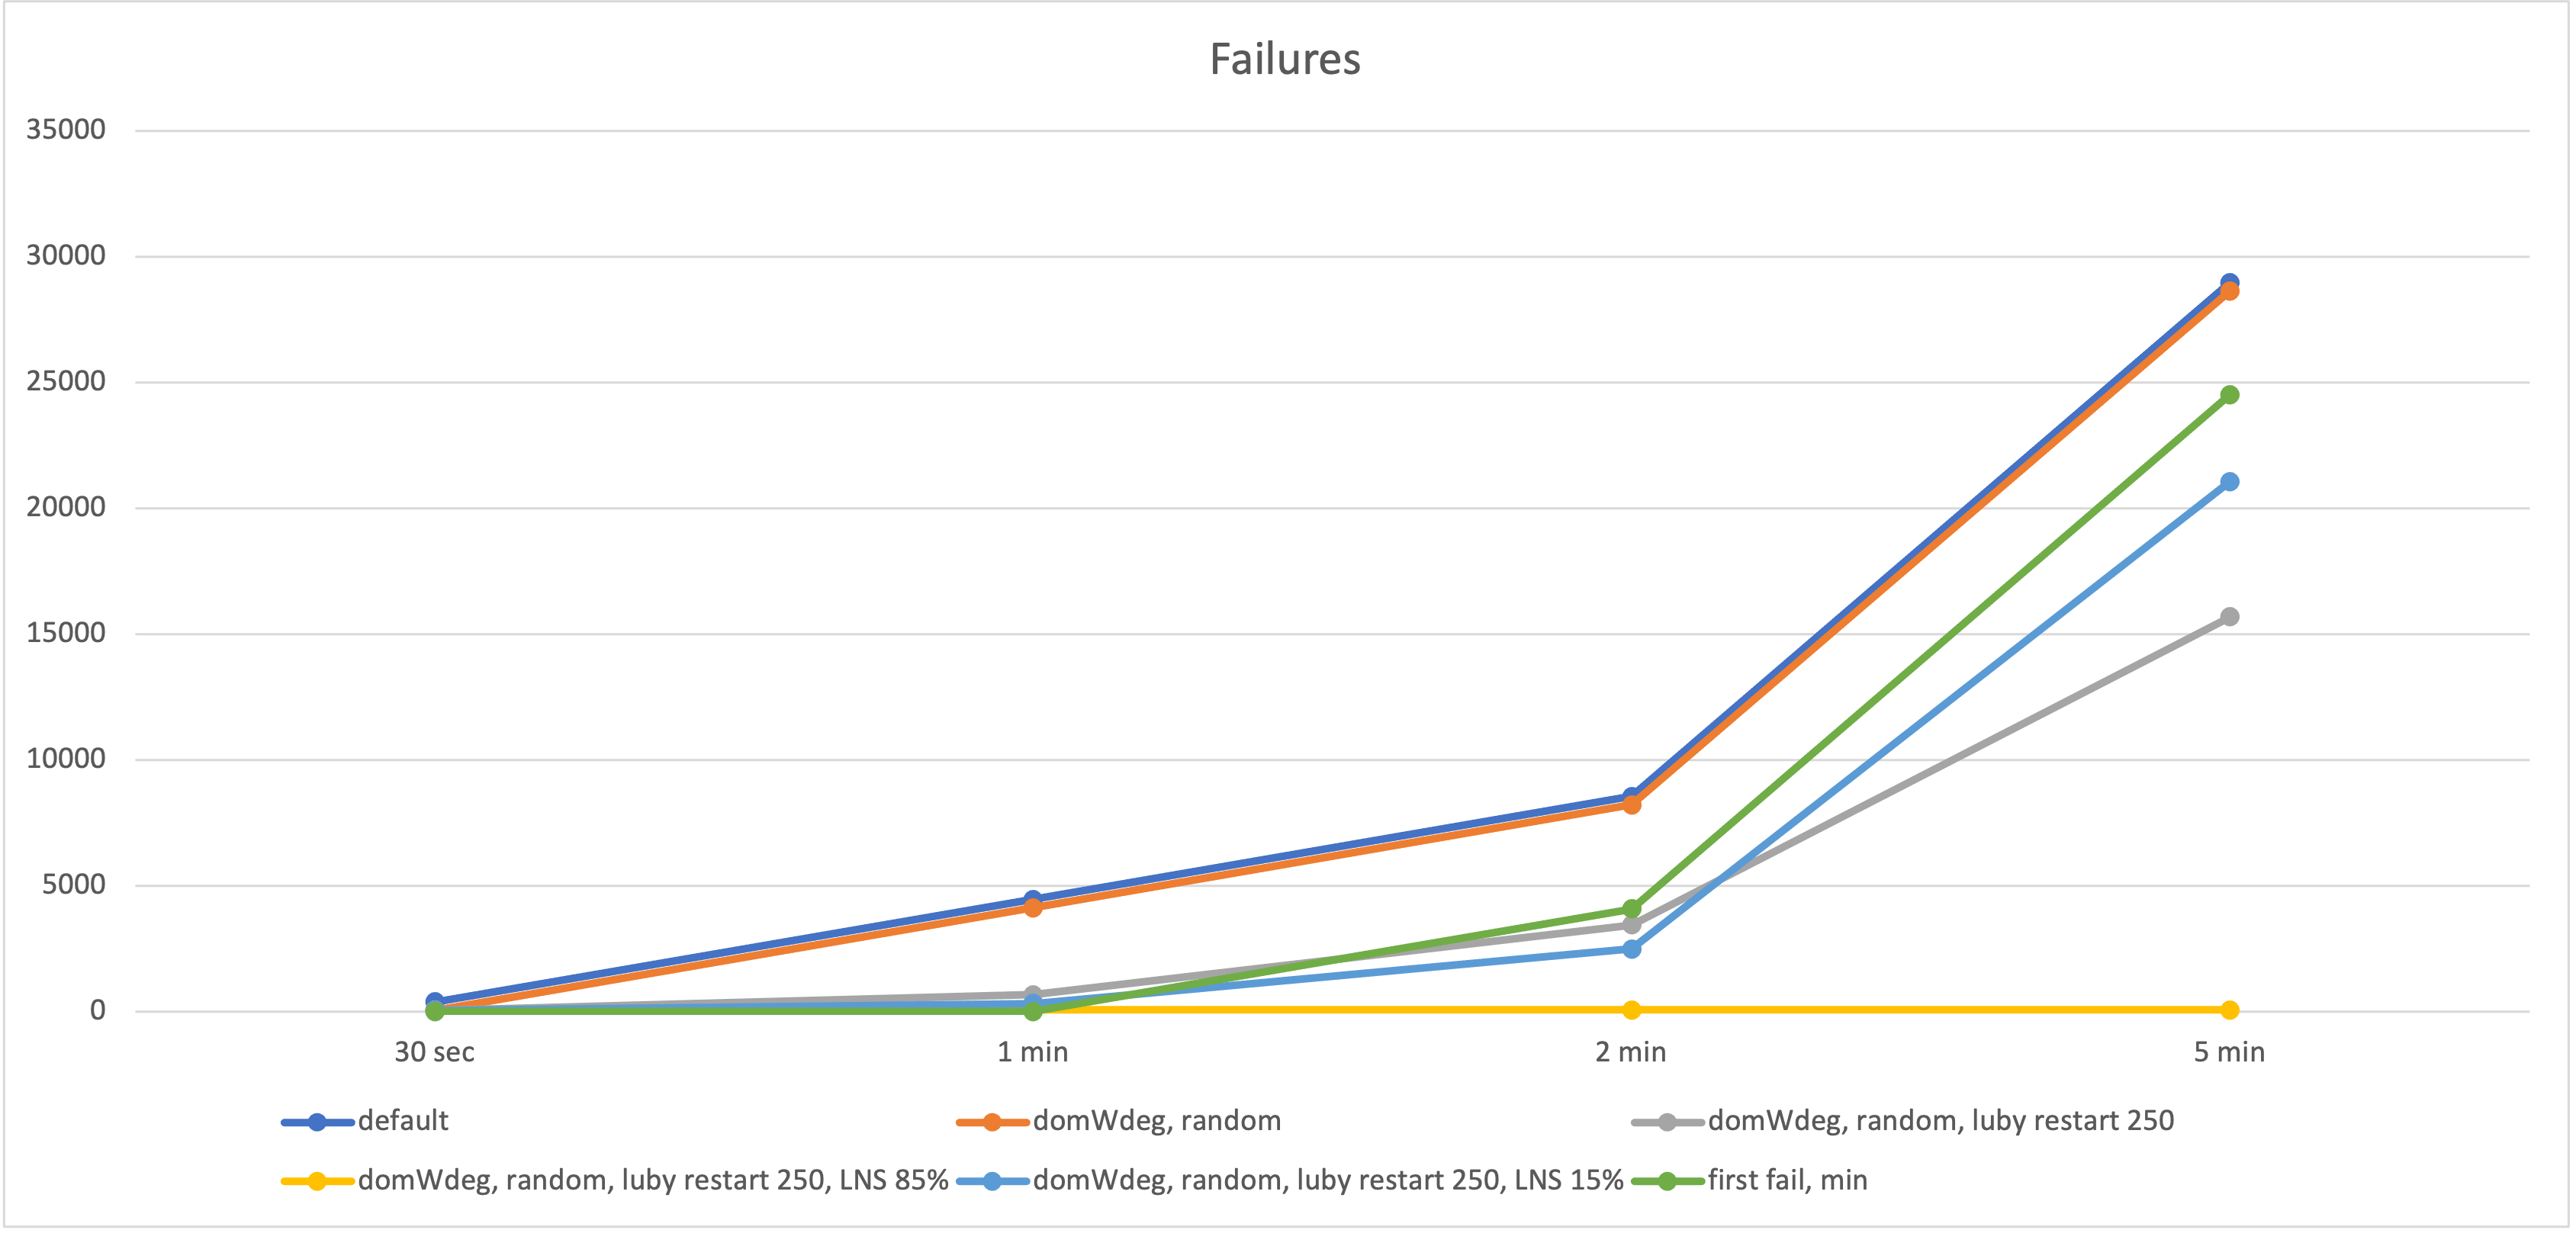
\includegraphics[width=1.0\columnwidth]{../graphs/pr09-failures.png}
    \caption{Failures graph for pr09.}
\end{figure}

{
\renewcommand{\arraystretch}{2}
\begin{longtable}[h]{| c | c | c | c | c |}
    \hline
    \textbf{Objective function} & \multicolumn{3}{c}{Time limit} & \\
    \hline
    \textbf{Search strategy} & \textbf{\textit{30 sec}} & \textbf{\textit{1 min}} & \textbf{\textit{2 min}} & \textbf{\textit{5 min}} \\
    \hline
    \endhead
    default search                                         & - & 169.220.760 & 168.356.810 & 167.182.710 \\
    \hline
    domWdeg, random                                        & - & 165.022.480 & 164.584.620 & 162.952.510 \\
    \hline
    domWdeg, random, Luby restart L=250                    & - & 155.316.990 & 155.316.990 & 154.486.560 \\
    \hline
    \textit{domWdeg, random, Luby restart L=250, LNS 85\%} & - & 155.316.990 & 154.734.780 & 153.642.510 \\
    \hline
    domWdeg, random, Luby restart L=250, LNS 15\%          & - & 155.316.990 & 155.316.990 & 153.990.910 \\
    \hline
    first fail, min                                        & - &         - & 163.015.510 & 160.750.880 \\
    \hline
\end{longtable}
}
\begin{figure}[H]
    \centering
    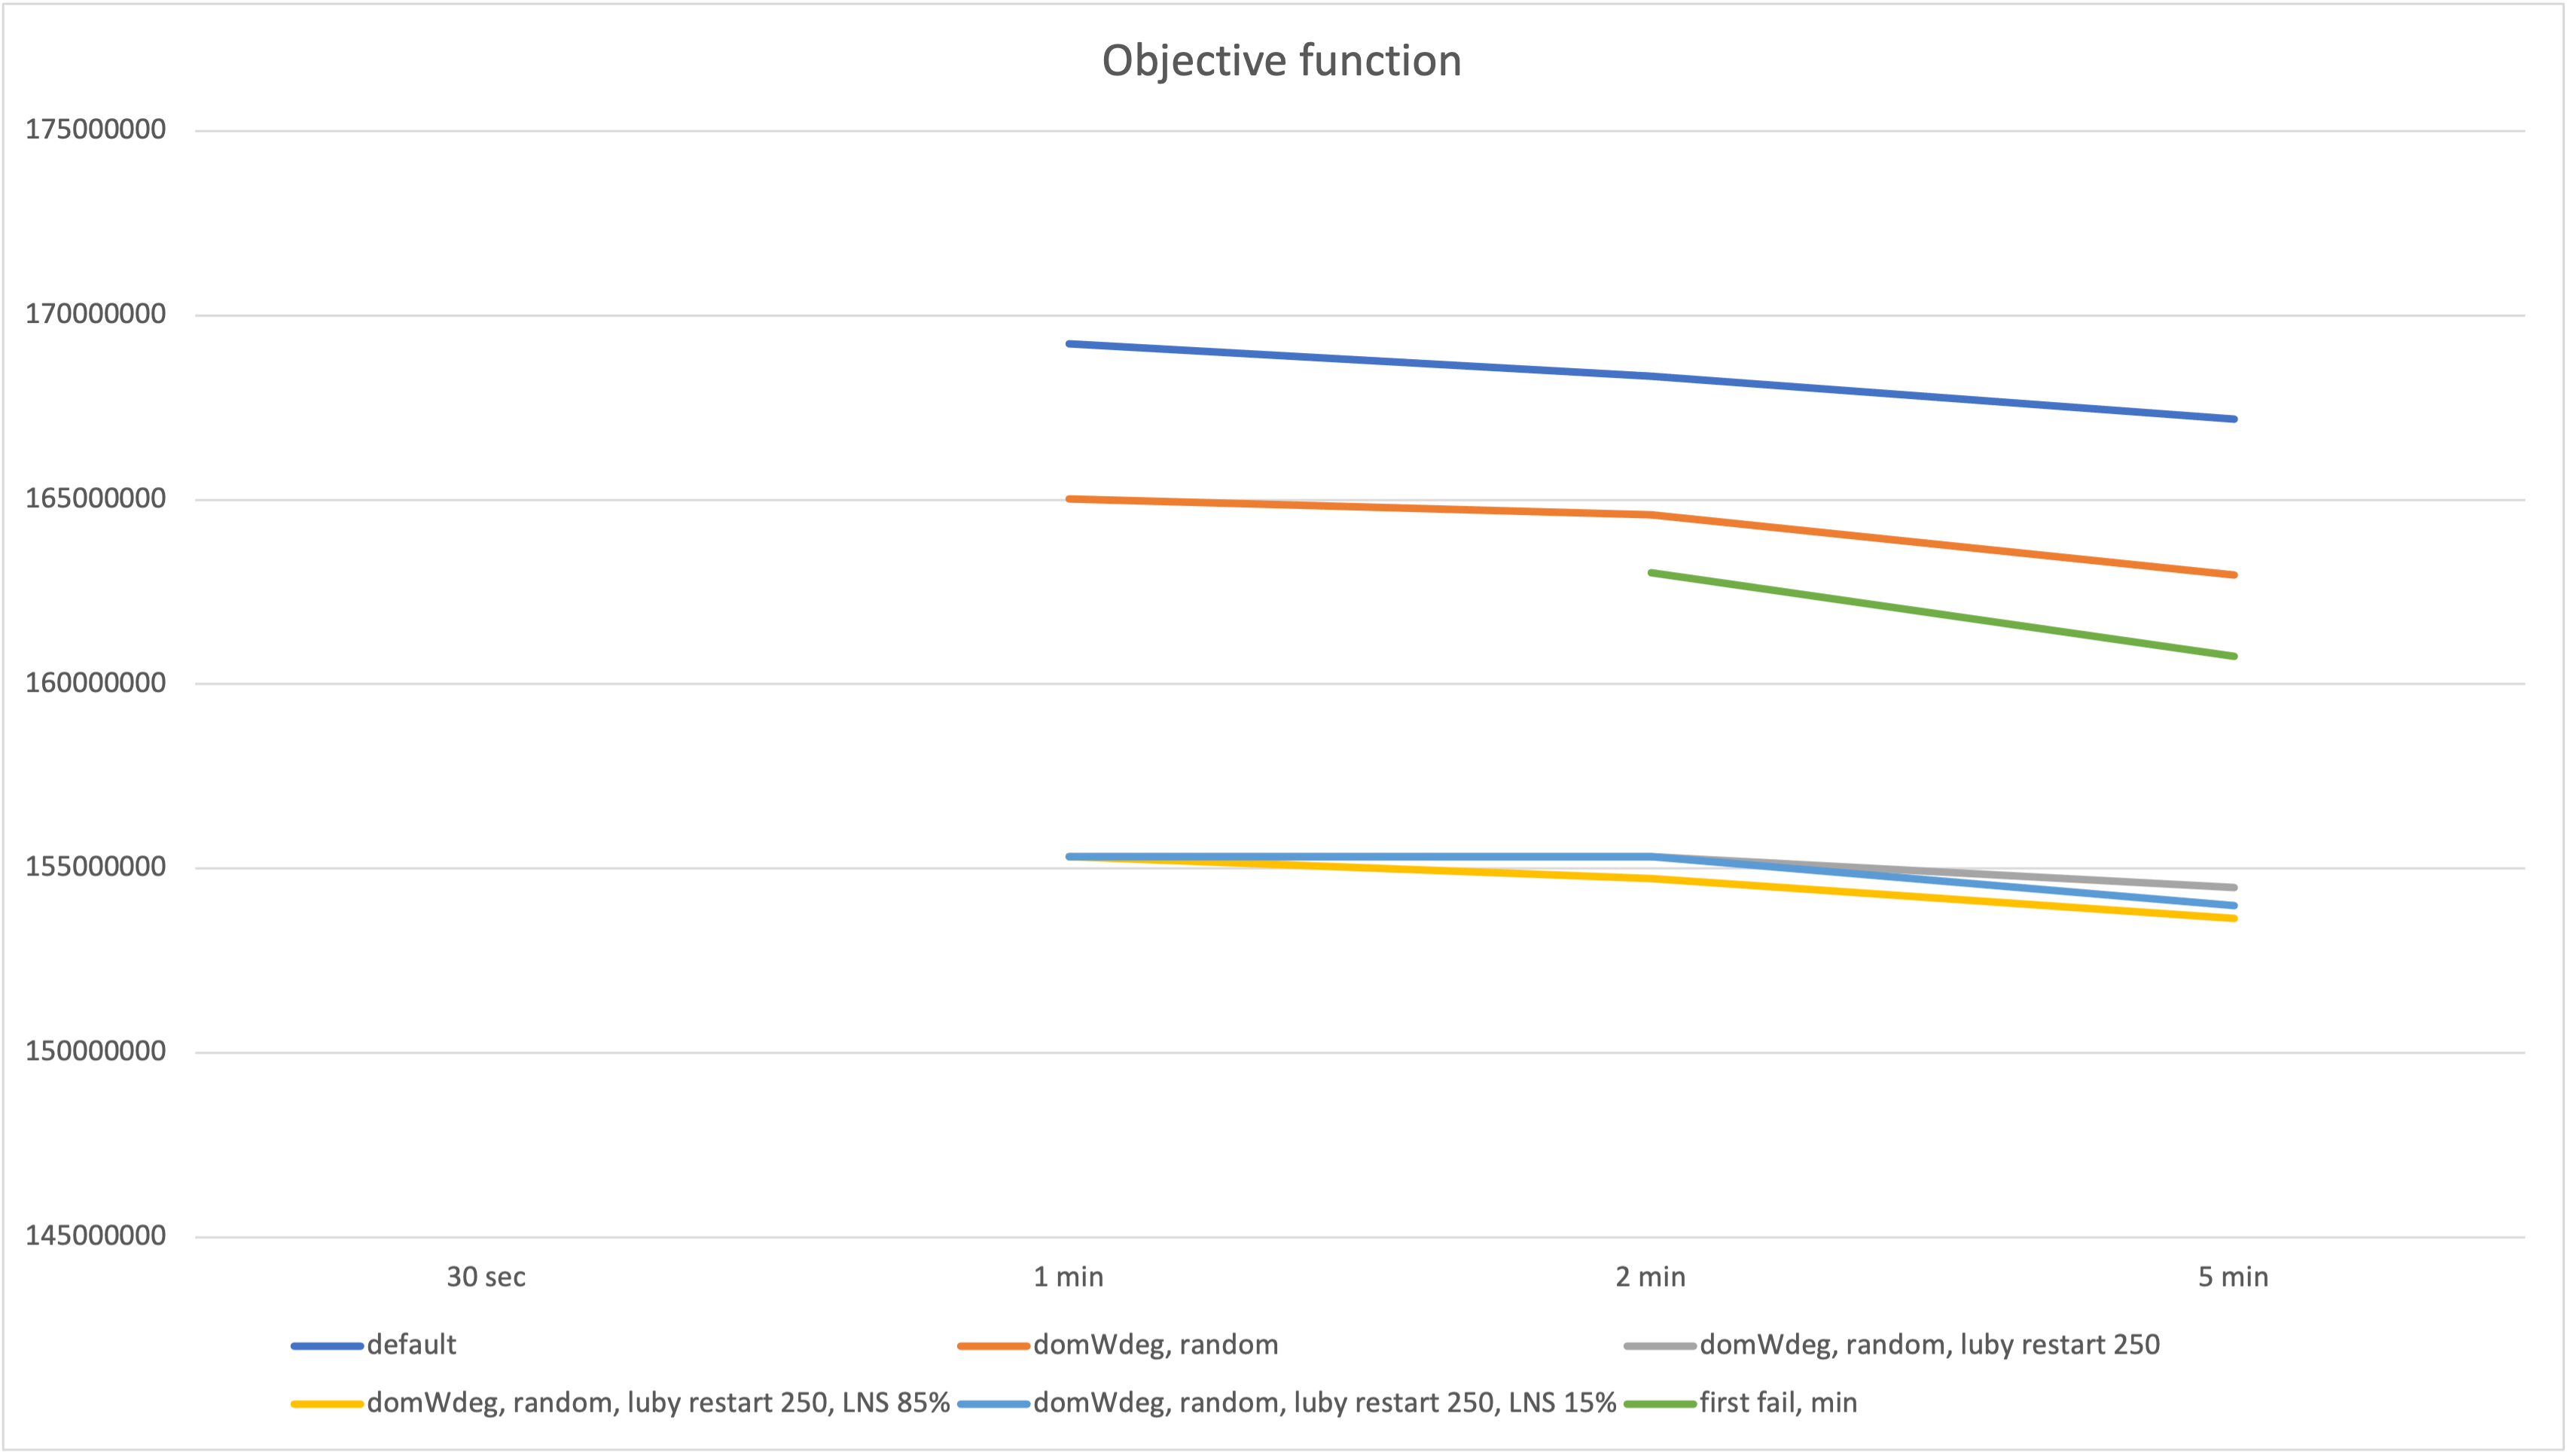
\includegraphics[width=1.0\columnwidth]{../graphs/pr09-objf.png}
    \caption{Objective functions graph for pr09.}
\end{figure}

{
\renewcommand{\arraystretch}{2}
\begin{longtable}[h]{| c | c | c | c |}
    \hline
    \textbf{Weights} & \textbf{Objective function} & \textbf{Total distance} & \textbf{Used vehicles} \\
    \hline
    \endhead
    $\alpha = 10, \beta = 0$ & 153.642.510 & 15.364.251 & 20 \\
    \hline
    $\alpha = 7, \beta = 3$  & 107.549.817 & 15.364.251 & 20 \\
    \hline
    $\alpha = 5, \beta = 5$  &  76.770.690 & 15.354.118 & 20 \\
    \hline
    $\alpha = 3, \beta = 7$  &  46.062.494 & 15.354.118 & 20 \\
    \hline
    $\alpha = 0, \beta = 10$ &         200 & 15.531.699 & 20 \\
    \hline
\end{longtable}
}
\begin{figure}[H]
    \centering
    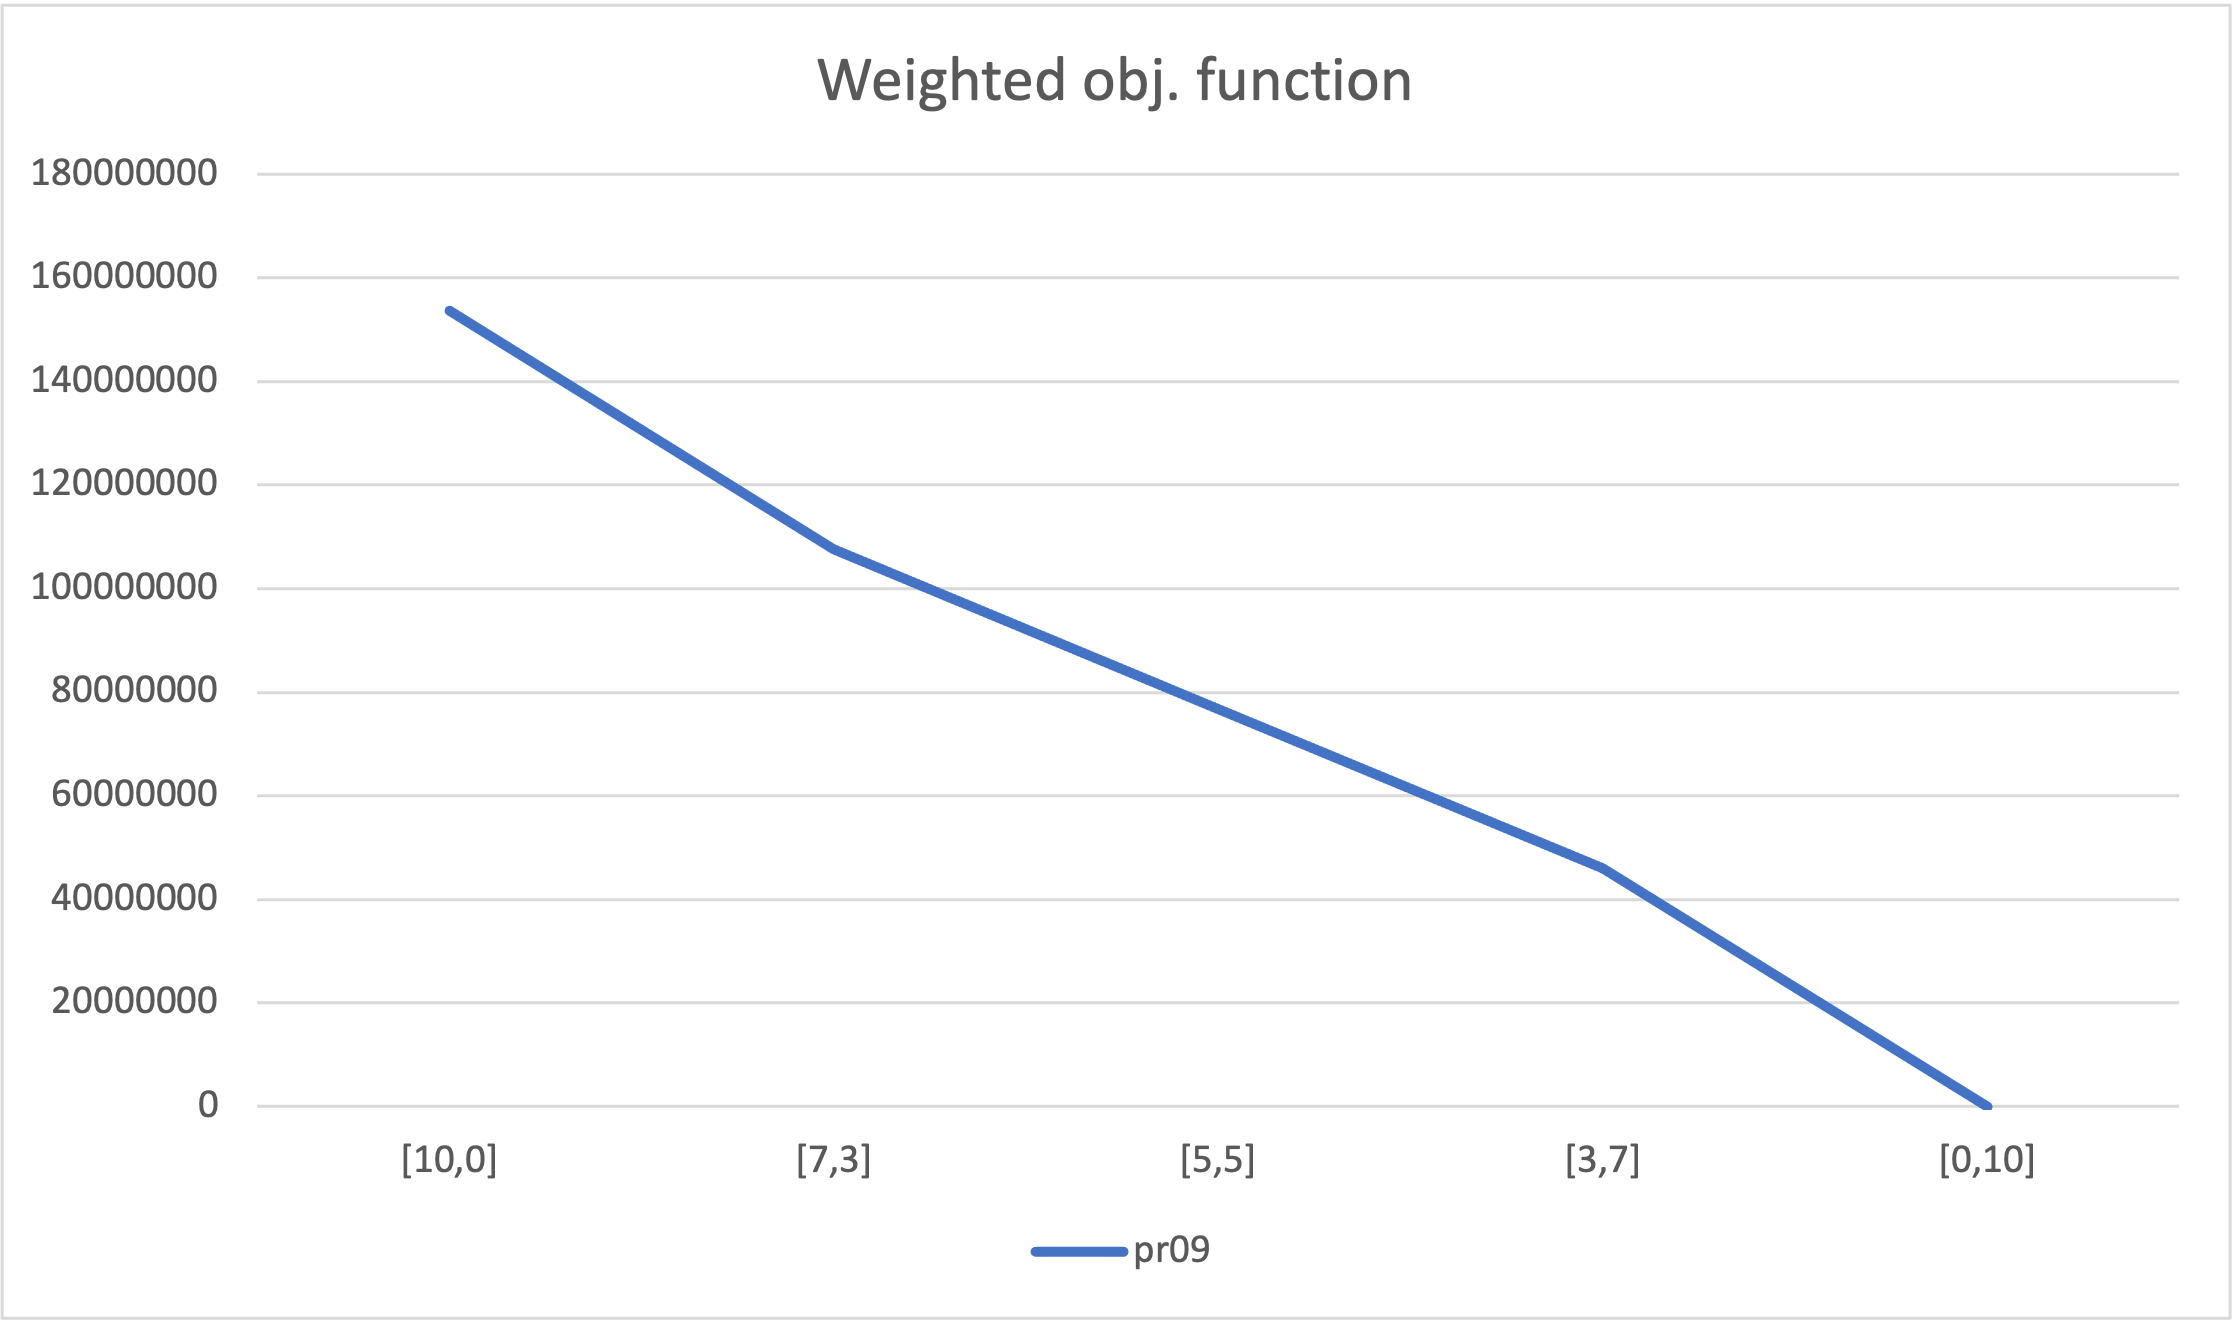
\includegraphics[width=1.0\columnwidth]{../graphs/pr09-wobjf.png}
    \caption{Weighted objective functions graph for pr09.}
\end{figure}

\begin{figure}[H]
    \centering
    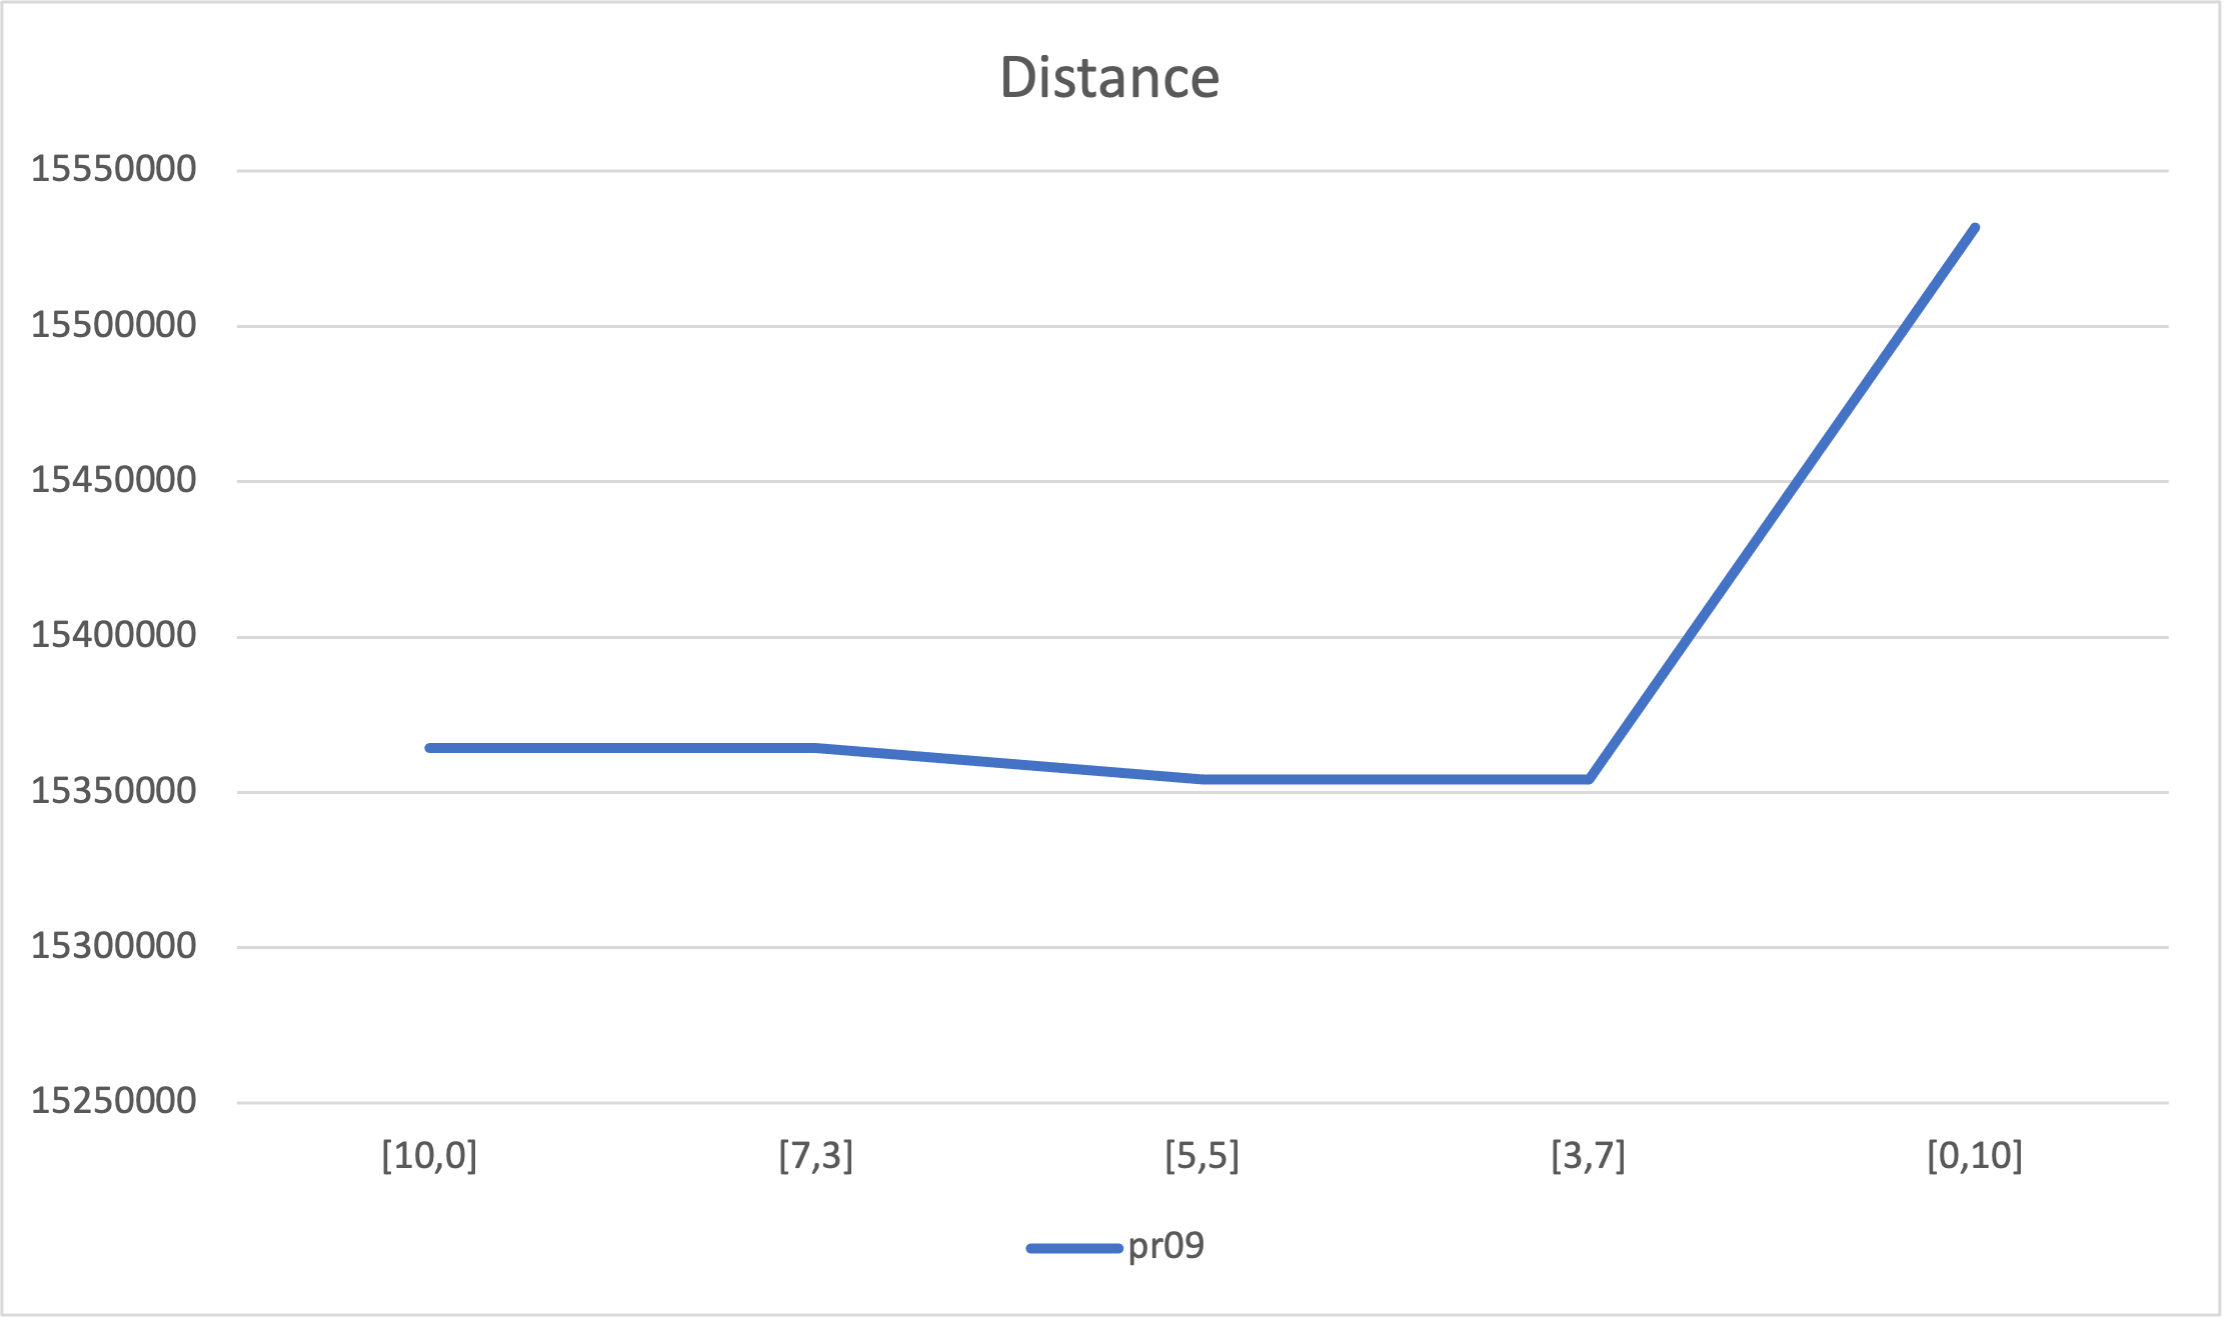
\includegraphics[width=1.0\columnwidth]{../graphs/pr09-distance.png}
    \caption{Distances graph for pr09.}
\end{figure}

\begin{figure}[H]
    \centering
    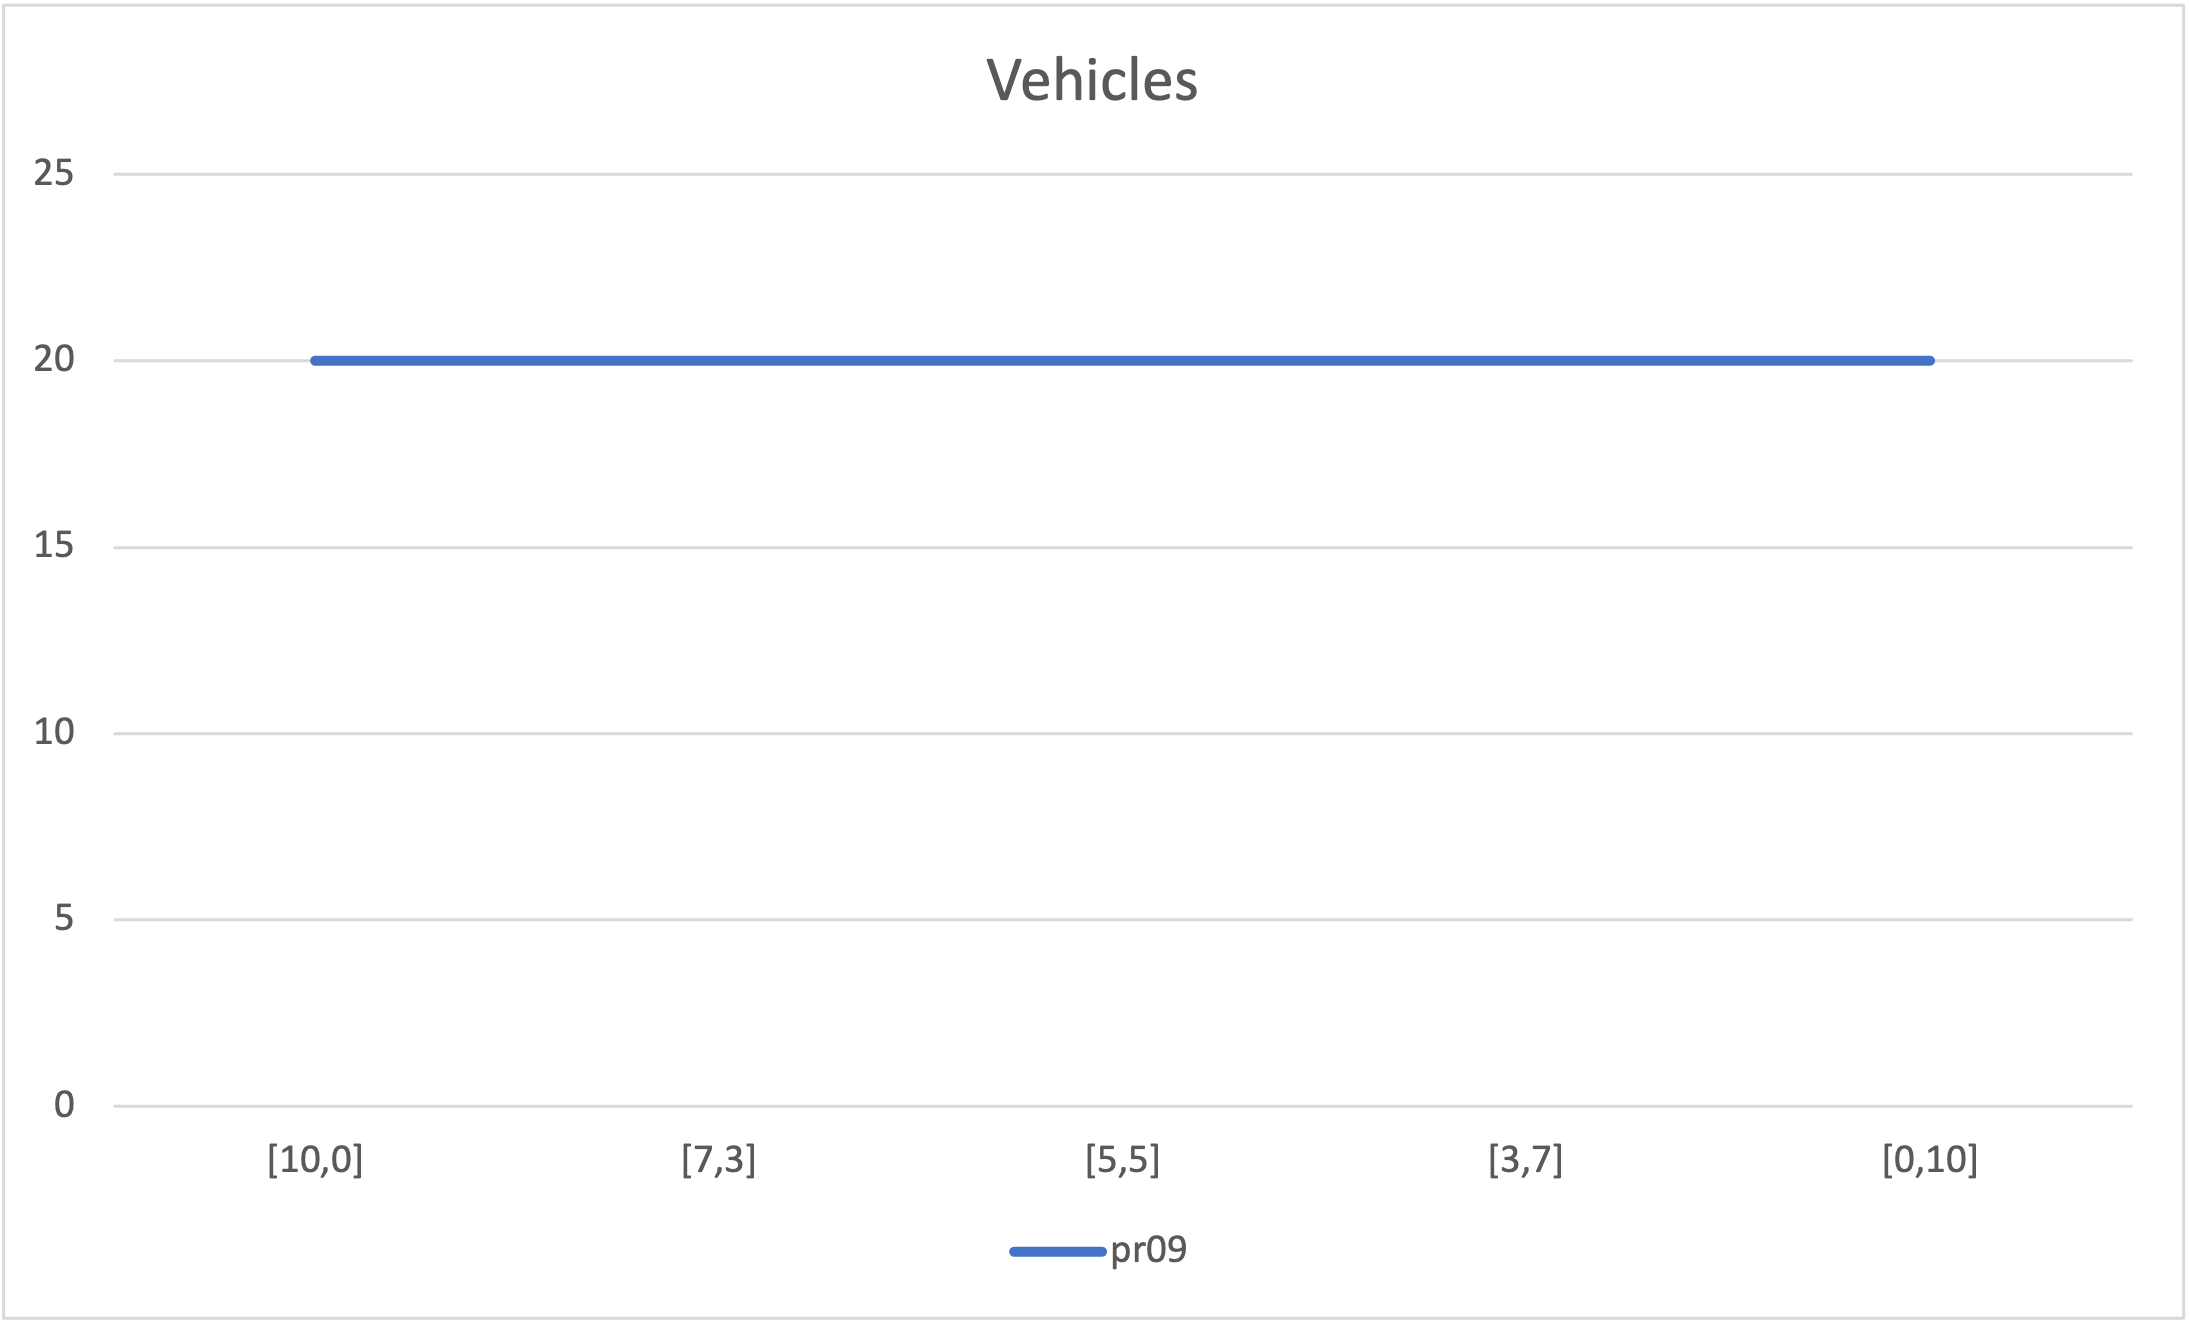
\includegraphics[width=1.0\columnwidth]{../graphs/pr09-vehicles.png}
    \caption{Vehicles used graph for pr09.}
\end{figure}
